%%%%%%%%%%%%%%%%%%%%%%%%%%%%%%%%%%%%%%%%%
% University/School Laboratory Report
% LaTeX Template
% Version 3.1 (25/3/14)
%
% This template has been downloaded from:
% http://www.LaTeXTemplates.com
%
% Original author:
% Linux and Unix Users Group at Virginia Tech Wiki 
% (https://vtluug.org/wiki/Example_LaTeX_chem_lab_report)
%
% License:
% CC BY-NC-SA 3.0 (http://creativecommons.org/licenses/by-nc-sa/3.0/)
%
%%%%%%%%%%%%%%%%%%%%%%%%%%%%%%%%%%%%%%%%%

%----------------------------------------------------------------------------------------
%	PACKAGES AND DOCUMENT CONFIGURATIONS
%----------------------------------------------------------------------------------------

\documentclass[12pt,a4paper,spanish]{article}
\usepackage[utf8]{inputenc}
\usepackage[T1]{fontenc}
\usepackage[version=3]{mhchem} % Package for chemical equation typesetting
\usepackage{siunitx} % Provides the \SI{}{} and \si{} command for typesetting SI units
\usepackage{graphicx} % Required for the inclusion of images
\usepackage{natbib} % Required to change bibliography style to APA
\usepackage{amsmath} % Required for some math elements 
\usepackage[table]{xcolor}
\usepackage{tikz}

\setlength\parindent{0pt} % Removes all indentation from paragraphs

\renewcommand{\labelenumi}{\alph{enumi}.} % Make numbering in the enumerate environment by letter rather than number (e.g. section 6)

%\usepackage{times} % Uncomment to use the Times New Roman font

%----------------------------------------------------------------------------------------
%	DOCUMENT INFORMATION
%----------------------------------------------------------------------------------------

\title{Actividad 4 \\ Logica Difusa} % Title


\date{\today} % Date for the report

\begin{document}

\maketitle % Insert the title, author and date


% If you wish to include an abstract, uncomment the lines below
% \begin{abstract}
% Abstract text
% \end{abstract}

%----------------------------------------------------------------------------------------
%	SECTION 1
%----------------------------------------------------------------------------------------

\clearpage
\section{Conjuntos difusos}
	\begin{itemize}
		\item 
		Entradas
		\begin{center}
		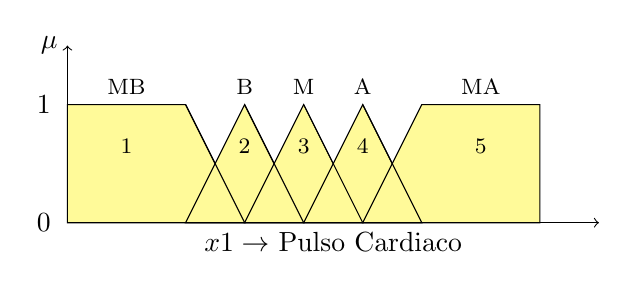
\begin{tikzpicture}[scale=1.5]

\begin{scope}[xshift=5.5cm]
\draw[->] (0,0) -- node[below] {$x1 \rightarrow$  Pulso Cardiaco} (4.5,0) ;
\draw[->] (0,0) -- (0,1.5) node[left] {$\mu$};
\node at (-0.2,0) {0};
\node at (-0.2,1) {1};
\draw[fill=yellow!40] (0,1) -- (1,1) -- (1.5,0) -- (0,0) -- (0,1) -- cycle;
\draw[fill=yellow!40] (1,0) -- (1.5,1) -- (2,0) -- (1,0) -- cycle;
\draw[fill=yellow!40] (1.5,0) -- (2,1) -- (2.5,0) -- (1.5,0) -- cycle;
\draw[fill=yellow!40] (2,0) -- (2.5,1) -- (3,0) -- (2,0) -- cycle;
\draw[fill=yellow!40] (2.5,0) -- (3,1) -- (4,1) -- (4,0) -- cycle;
\draw (1,1) -- (1.5,0);
\draw (1.5,1) -- (2,0);
\draw (2,1) -- (2.5,0);
\draw (2.5,1) -- (3,0);
\node[above,font=\footnotesize] at (0.5,1) {MB};
\node[above,font=\footnotesize] at (1.5,1) {B};
\node[above,font=\footnotesize] at (2,1) {M};
\node[above,font=\footnotesize] at (2.5,1) {A};
\node[above,font=\footnotesize] at (3.5,1) {MA};
\node[above,font=\footnotesize] at (0.5,0.5) {1};
\node[above,font=\footnotesize] at (1.5,0.5) {2};
\node[above,font=\footnotesize] at (2,0.5) {3};
\node[above,font=\footnotesize] at (2.5,0.5) {4};
\node[above,font=\footnotesize] at (3.5,0.5) {5};
\end{scope}

\end{tikzpicture}

	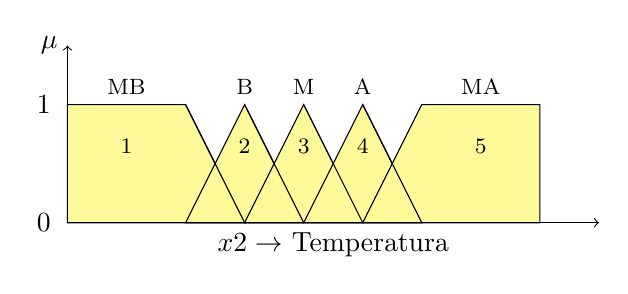
\begin{tikzpicture}[scale=1.5]

\begin{scope}[xshift=5.5cm]
\draw[->] (0,0) -- node[below] {$x2 \rightarrow$ Temperatura} (4.5,0) ;
\draw[->] (0,0) -- (0,1.5) node[left] {$\mu$};
\node at (-0.2,0) {0};
\node at (-0.2,1) {1};
\draw[fill=yellow!40] (0,1) -- (1,1) -- (1.5,0) -- (0,0) -- (0,1) -- cycle;
\draw[fill=yellow!40] (1,0) -- (1.5,1) -- (2,0) -- (1,0) -- cycle;
\draw[fill=yellow!40] (1.5,0) -- (2,1) -- (2.5,0) -- (1.5,0) -- cycle;
\draw[fill=yellow!40] (2,0) -- (2.5,1) -- (3,0) -- (2,0) -- cycle;
\draw[fill=yellow!40] (2.5,0) -- (3,1) -- (4,1) -- (4,0) -- cycle;
\draw (1,1) -- (1.5,0);
\draw (1.5,1) -- (2,0);
\draw (2,1) -- (2.5,0);
\draw (2.5,1) -- (3,0);
\node[above,font=\footnotesize] at (0.5,1) {MB};
\node[above,font=\footnotesize] at (1.5,1) {B};
\node[above,font=\footnotesize] at (2,1) {M};
\node[above,font=\footnotesize] at (2.5,1) {A};
\node[above,font=\footnotesize] at (3.5,1) {MA};
\node[above,font=\footnotesize] at (0.5,0.5) {1};
\node[above,font=\footnotesize] at (1.5,0.5) {2};
\node[above,font=\footnotesize] at (2,0.5) {3};
\node[above,font=\footnotesize] at (2.5,0.5) {4};
\node[above,font=\footnotesize] at (3.5,0.5) {5};
\end{scope}

\end{tikzpicture}

	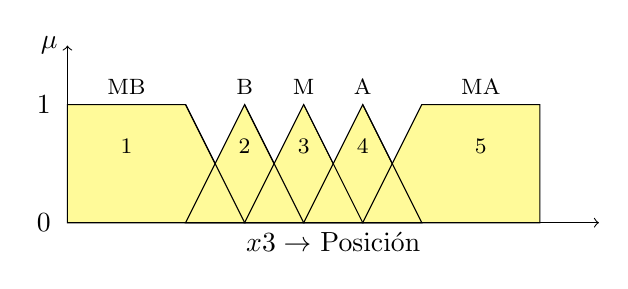
\begin{tikzpicture}[scale=1.5]

\begin{scope}[xshift=5.5cm]
\draw[->] (0,0) -- node[below] {$x3 \rightarrow$ Posición} (4.5,0);
\draw[->] (0,0) -- (0,1.5) node[left] {$\mu$};
\node at (-0.2,0) {0};
\node at (-0.2,1) {1};
\draw[fill=yellow!40] (0,1) -- (1,1) -- (1.5,0) -- (0,0) -- (0,1) -- cycle;
\draw[fill=yellow!40] (1,0) -- (1.5,1) -- (2,0) -- (1,0) -- cycle;
\draw[fill=yellow!40] (1.5,0) -- (2,1) -- (2.5,0) -- (1.5,0) -- cycle;
\draw[fill=yellow!40] (2,0) -- (2.5,1) -- (3,0) -- (2,0) -- cycle;
\draw[fill=yellow!40] (2.5,0) -- (3,1) -- (4,1) -- (4,0) -- cycle;
\draw (1,1) -- (1.5,0);
\draw (1.5,1) -- (2,0);
\draw (2,1) -- (2.5,0);
\draw (2.5,1) -- (3,0);
\node[above,font=\footnotesize] at (0.5,1) {MB};
\node[above,font=\footnotesize] at (1.5,1) {B};
\node[above,font=\footnotesize] at (2,1) {M};
\node[above,font=\footnotesize] at (2.5,1) {A};
\node[above,font=\footnotesize] at (3.5,1) {MA};
\node[above,font=\footnotesize] at (0.5,0.5) {1};
\node[above,font=\footnotesize] at (1.5,0.5) {2};
\node[above,font=\footnotesize] at (2,0.5) {3};
\node[above,font=\footnotesize] at (2.5,0.5) {4};
\node[above,font=\footnotesize] at (3.5,0.5) {5};
\end{scope}

\end{tikzpicture}
	\end{center}
	\item
		Salidas
		\begin{center}
			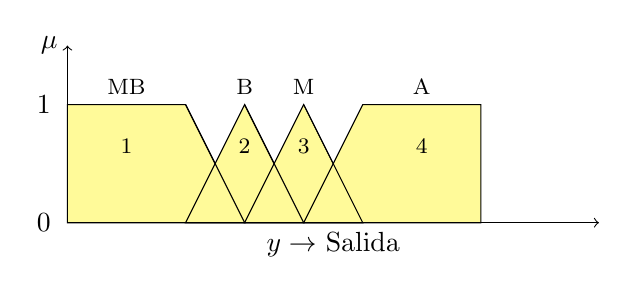
\begin{tikzpicture}[scale=1.5]

\begin{scope}[xshift=5.5cm]
\draw[->] (0,0) -- node[below] {$y \rightarrow$ Salida} (4.5,0);
\draw[->] (0,0) -- (0,1.5) node[left] {$\mu$};
\node at (-0.2,0) {0};
\node at (-0.2,1) {1};
\draw[fill=yellow!40] (0,1) -- (1,1) -- (1.5,0) -- (0,0) -- (0,1) -- cycle;
\draw[fill=yellow!40] (1,0) -- (1.5,1) -- (2,0) -- (1,0) -- cycle;
\draw[fill=yellow!40] (1.5,0) -- (2,1) -- (2.5,0) -- (1.5,0) -- cycle;
\draw[fill=yellow!40] (2,0) -- (2.5,1) -- (3.5,1) -- (3.5,0) -- (2,0) -- cycle;
\draw (1,1) -- (1.5,0);
\draw (1.5,1) -- (2,0);
\draw (2,1) -- (2.5,0);
\draw (2.5,1) -- (3.5,1);
\node[above,font=\footnotesize] at (0.5,1) {MB};
\node[above,font=\footnotesize] at (1.5,1) {B};
\node[above,font=\footnotesize] at (2,1) {M};
\node[above,font=\footnotesize] at (3,1) {A};
\node[above,font=\footnotesize] at (0.5,0.5) {1};
\node[above,font=\footnotesize] at (1.5,0.5) {2};
\node[above,font=\footnotesize] at (2,0.5) {3};
\node[above,font=\footnotesize] at (3,0.5) {4};
\end{scope}

\end{tikzpicture}
		\end{center}
		
	\end{itemize}
	
	
\clearpage
\section{Reglas Difusas}


%----------------------------------------------------------------------------------------
%	BIBLIOGRAPHY
%----------------------------------------------------------------------------------------

\bibliographystyle{apalike}

\bibliography{sample}

%----------------------------------------------------------------------------------------


\end{document}